%
\begin{figure}[t!]
\centering
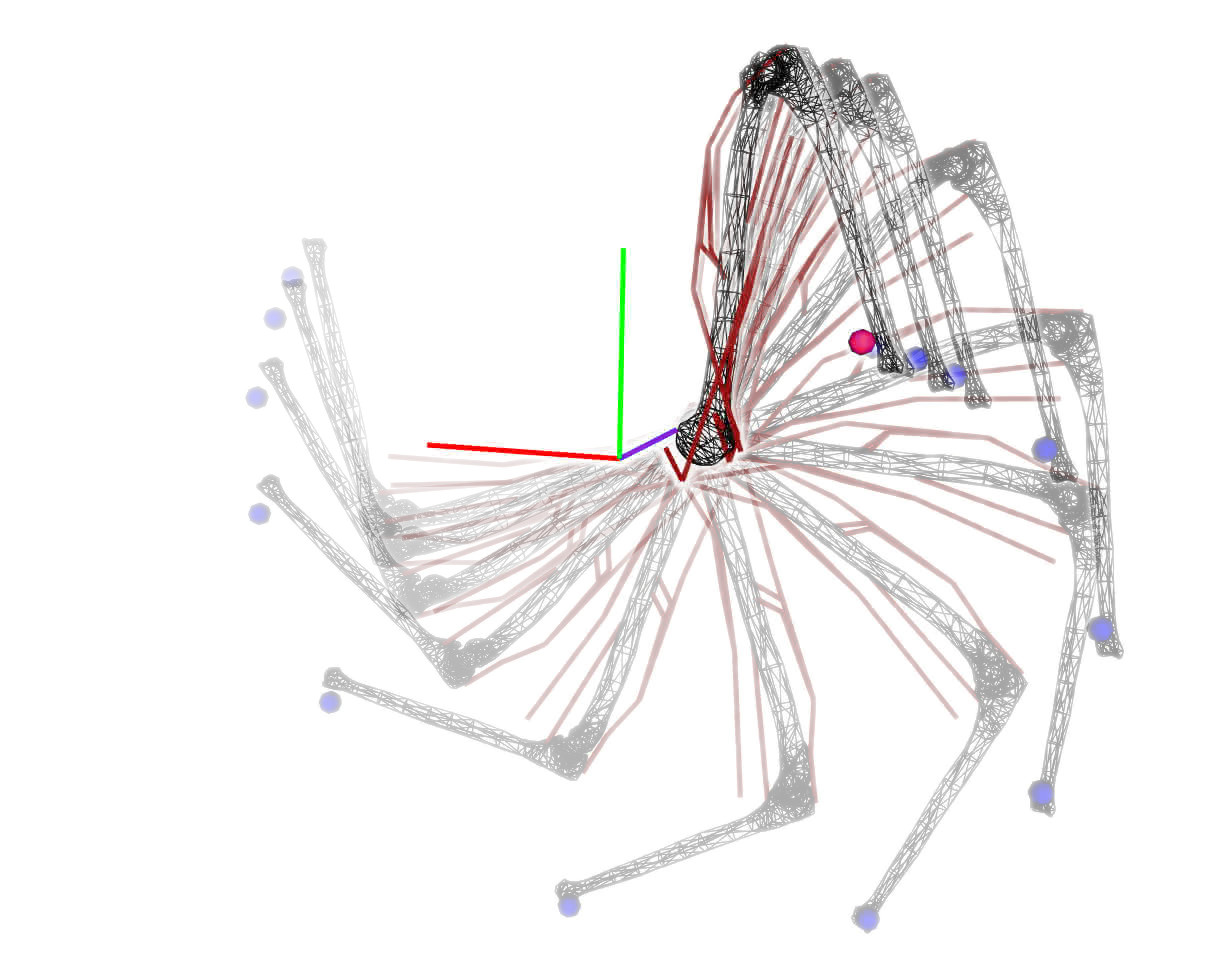
\includegraphics[width=\columnwidth]{figures/activation_pointing.jpeg}\\
\caption{Snapshots of an optimized activation-driven pointing task with \acados. The arm starts facing upwards in left hand part of the picture and ends facing downwards in the right hand part. The marker fixed on the ulna head is depicted in blue and the scene-fixed target marker is depicted in red. Red lines show the lines of actions of the muscles.}
\label{fig:snapshots_activation_driven_pointing}
\vspace*{-0.5cm}
\end{figure}
\begin{figure*}[t!]
\centering
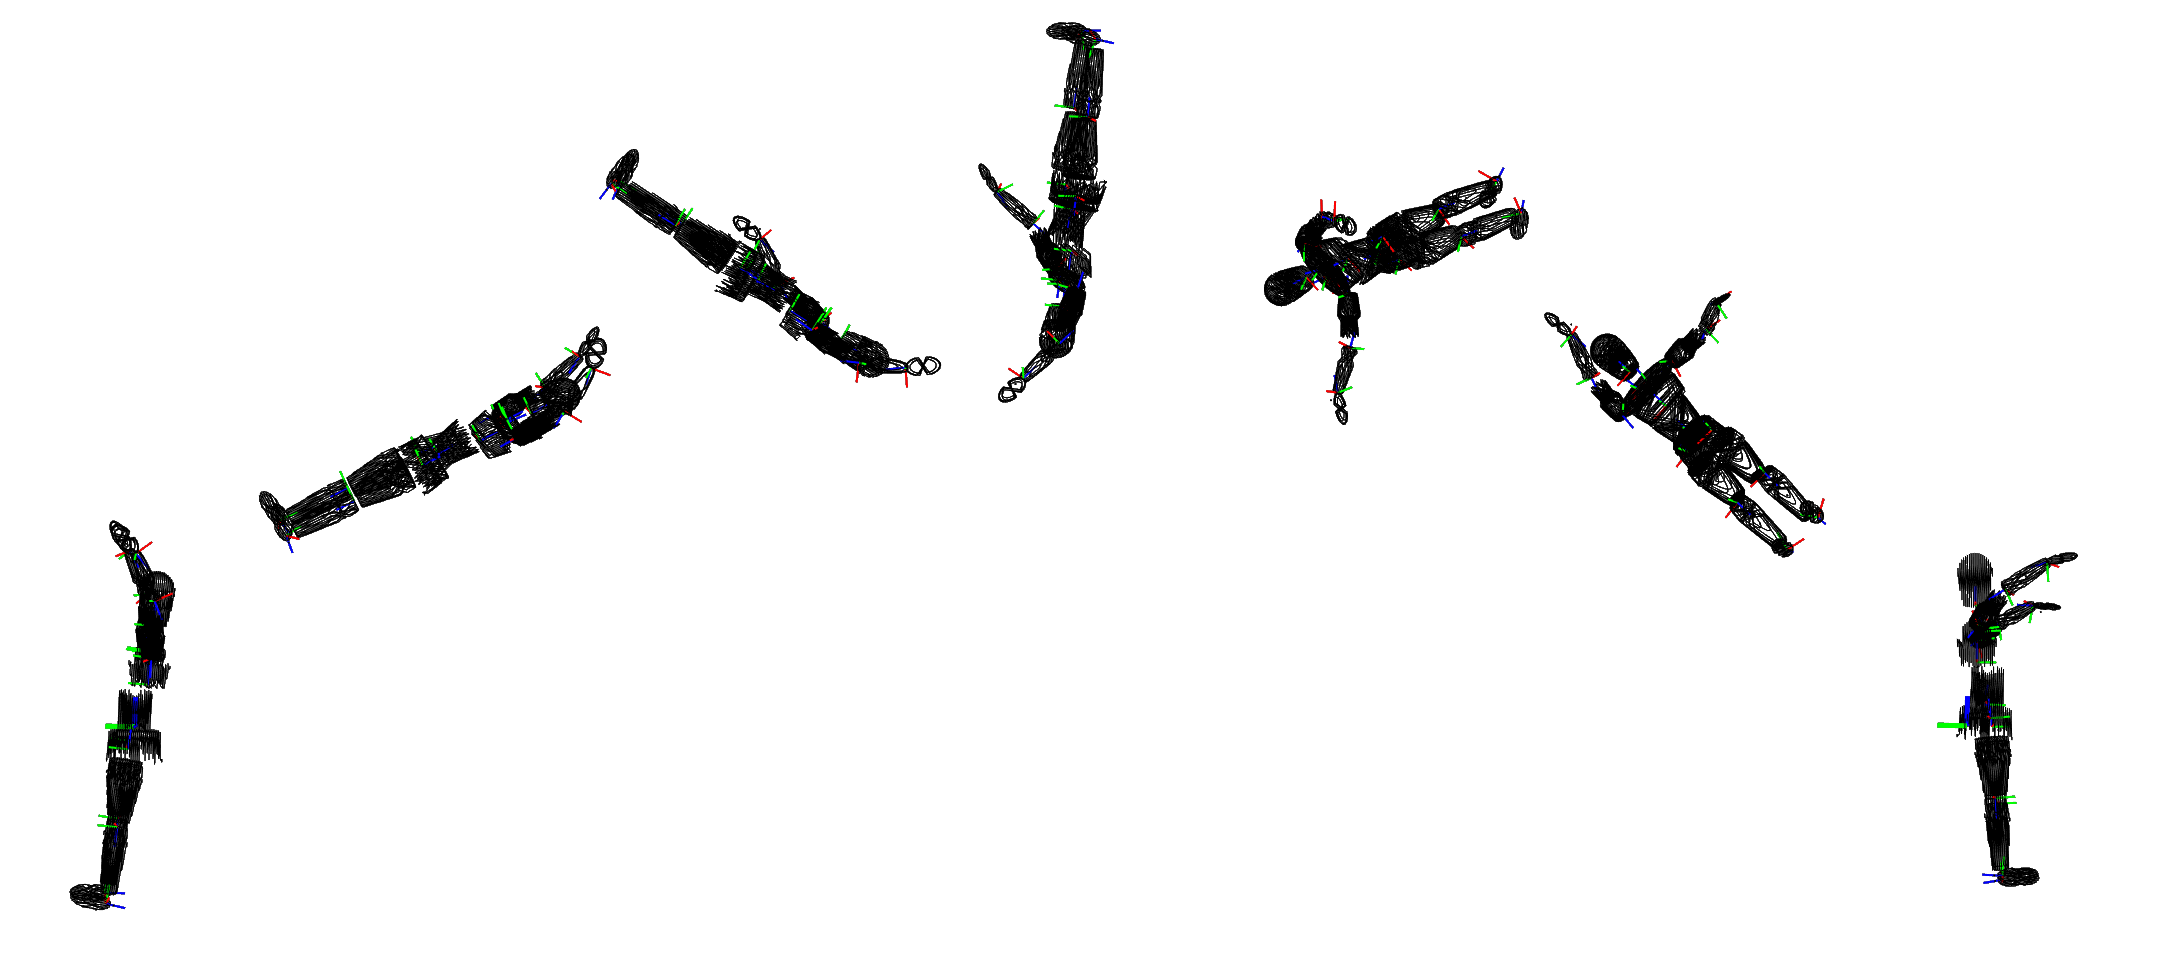
\includegraphics[width=\textwidth]{figures/Euler_Bioptim_MaxVrille_dos_7frames.png}
\caption{Snapshots of maximally twisting somersaults driven by shoulder torque actuators and a free base whose rotation is either expressed by Euler angles (top) or by quaternions (bottom).}
\label{fig:snapshots_quaternion_base_twisting_somersault}
\end{figure*}
%
In this first example, the goal was to achieve a muscle activation driven pointing task using a 2-DoF arm model with six muscle elements. 
In addition to muscle-induced torques, pure joint torques were added to compensate for the model weaknesses.
The main term (highest weight) of the objective function (Eq.~\ref{eq:cost_pointing}) is a Mayer objective, corresponding to the pointing tasks at the final node, to superimpose two markers, the first one ($\mathbf{m_u}$) fixed in the ulna system of coordinates and the second one ($\mathbf{m^*_s}$) fixed in the scene.
The three Lagrange terms  were added for control (muscle activation $\bf{a}$ and joint torques $\boldsymbol{\tau}$) and state ($\bf{x}$) regularization:
\[
\begin{aligned}
	\mathcal{J} = 	&~\omega_1~\underbrace{\|\mathbf{m_u}(T)-\mathbf{m^*_s}\|^2}_{\mathtt{TRACK\_MARKERS}}~\\
	&\int_{t=0}^T\underbrace{\|\bf{a}\|^2}_{\mathtt{MIN\_ACTIVATION}}~
	+\underbrace{\|\boldsymbol\tau\|^2}_{\mathtt{MIN\_TORQUE}}~
	+\underbrace{\|\bf{x}\|^2}_{\mathtt{MIN\_STATE}}~ dt,
\end{aligned}
\addtag
\label{eq:cost_pointing}
\]

\noindent where $T\!=\!\SI{2}{\second}$ is the duration of the motion, and $\omega_1\!=\!1e5$.
The problem was discretized using 50~shooting nodes with a 5-steps RK4 integration in-between.
The problem was solved using \ipopt (with exact Hessian computations) and \acados (with a Gauss-Newton approximation of the Hessian) resulting in two very close solutions.
\acados was about 50 times faster than \ipopt and was better at enforcing the continuity constraints (as shown by the single shooting error in Tab.~\ref{tab:Perfs_and_detailed_implementations_of_each_example}).
\ipopt however ended up with a smaller optimized objective (20.8 \textit{vs} 23.2), leading to a more optimal solution than \acados. 
Superimposed snapshots of the optimal motion found with \acados are displayed in Fig.~\ref{fig:snapshots_activation_driven_pointing}.
It is worth mentioning that for the purpose of this illustration, no constraint was given on the shoulder range of motion to ensure physiological muscle trajectories. 








